\documentclass{article}
%\usepackage{pgfplots}
%\usepackage{graphicx}
\usepackage{amsmath}
\usepackage{amsfonts}
\usepackage{mathtools}
\usepackage{pgfplots}
\usepackage{graphicx}
\usepackage[english]{babel}
\author{Yiqing(Alice) Guo}
\title{Assignment 1\\ \large CSCI-6390}

\begin{document}
\maketitle
\paragraph{}For all part that all results have precision of 8
\paragraph{read me\\}
python version:  2.7.11
\\sample command line input: assign1.py airfoil\_self\_noise.dat 8 0.0001 out.txt
\\python file, data file, precision, epsilon, output file
\\all print text result are save in out.txt
\\if there are no 5 argument then the output will print in the command windows.
\\sample command line input with 4 arguments: assign1.py airfoil\_self\_noise.dat 8 0.0001
\\if less than 4 argument then the code will using the defualt value.
\\4 figure are saved as most\_correlated.png, anti\_correlated.png, least\_correlated.png, eigenvectors.png 
\section{Part 1}
\paragraph{Compute the mean vector $\mu$ for the 6-dimensional data matrix, and then compute the total variance  $var(D)$}
\subparagraph{}The mean vector $\mu$: \[ 
\begin{bmatrix}2886.38057219  &   6.78230206 &    0.13654824   & 50.86074518    & 0.01113988
   &124.83594278\end{bmatrix}\]
\subparagraph{}Total variance  $var(D)$: $9932429.7172$
\paragraph{Compute the sample covariance matrix $\Sigma$ as inner products between the attributes of the centered data matrix.Next compute the sample covariance matrix as sum of the outer products between the centered points}
\subparagraph{}Inner products:\[ 
\begin{bmatrix}9932104.79728063   & -5085.67250617   &    -1.07878216    & 6557.77175899
     &   -9.53323084  &  -8491.74115188\\
  -5085.67250617    &   35.00093761     &  -0.27930199     &   5.41178032
      &   0.05859369      & -6.36918252\\
    -1.07878216     &  -0.27930199      &  0.00874405       & 0.00551227
       & -0.00027147     &  -0.1522949 \\
   6557.77175899   &     5.41178032   &     0.00551227   &   242.35026212
     &   -0.00081328  &     13.43101346\\
       -9.53323084& 0.05859369& -0.00027147& -0.00081328
& 0.00017281& -0.02834618\\
  -8491.74115188&       -6.36918252  &     -0.1522949 &       13.43101346
    &    -0.02834618    &   47.55979887\end{bmatrix}\]
\subparagraph{}Outer products:\[ 
\begin{bmatrix}9932104.79728063   & -5085.67250617   &    -1.07878216    & 6557.77175899
     &   -9.53323084  &  -8491.74115188\\
  -5085.67250617    &   35.00093761     &  -0.27930199     &   5.41178032
      &   0.05859369      & -6.36918252\\
    -1.07878216     &  -0.27930199      &  0.00874405       & 0.00551227
       & -0.00027147     &  -0.1522949 \\
   6557.77175899   &     5.41178032   &     0.00551227   &   242.35026212
     &   -0.00081328  &     13.43101346\\
       -9.53323084& 0.05859369& -0.00027147& -0.00081328
& 0.00017281& -0.02834618\\
  -8491.74115188&       -6.36918252  &     -0.1522949 &       13.43101346
    &    -0.02834618    &   47.55979887\end{bmatrix}\]
\paragraph{Compute the correlation matrix for this dataset using the formula for the cosine between centered attribute vectors.Which attributes are the most correlated, the most anti-correlated, and least correlated? Create the scatter plots for these interesting pairs using matplotlib and visually confirm the trends, i.e., describe how each of the three cases results in a particular type of plot.}
\begin{center}
\begin{tabular}{| l | l | l | l | l |}
\hline
Colume & Colume  & $cos(\theta)$  & Degree\\ \hline
1& 1&1.000000&0.00\\ \hline
1&2&-0.272765&105.83\\ \hline
1& 3&-0.003661&90.21\\ \hline
1& 4&0.133664&82.32\\ \hline
1& 5&-0.230107&103.30\\ \hline
1& 6&-0.390711&113.00\\ \hline
2& 2&1.000000&0.00\\ \hline
2& 3&-0.504868&120.32\\ \hline
2& 4&0.058760&86.63\\ \hline
2& 5&0.753394&41.11\\ \hline
2& 6&-0.156108&98.98\\ \hline
3& 3&1.000000&0.00\\ \hline
3& 4&0.003787&89.78\\ \hline
3& 5&-0.220842&102.76\\ \hline
3& 6&-0.236162&103.66\\ \hline
4& 4&1.000000&0.00\\ \hline
4&5&-0.003974&90.23\\ \hline
4& 6&0.125103&82.81\\ \hline
5& 5&1.000000&0.00\\ \hline
5&6&-0.312670&108.22\\ \hline
6& 6&1.000000&0.00\\ \hline
\end{tabular}
\end{center}
\subparagraph{}The most correlated is col: (2, 5) , $cos(\theta)$ is 0.753394, and the degree is 41.11
\subparagraph{}In this we see that one variable increases, the other tends to also increase. we could see a positive relation ship between the two attribute.
\subparagraph{}
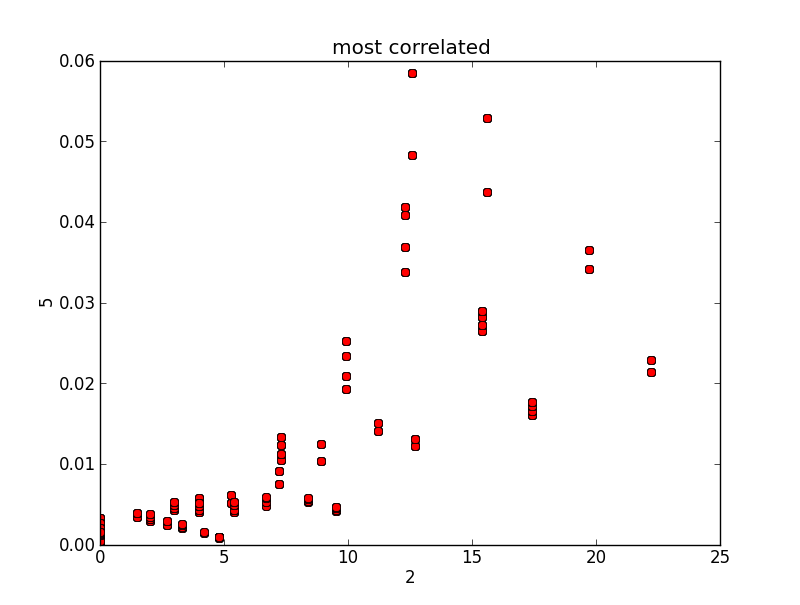
\includegraphics[scale=0.5]{figure_1}
\subparagraph{}The most anti-correlated is col: (2, 3) , $cos(\theta)$ is  -0.504868, and the degree is 120.32
\subparagraph{}In this we see that one variable increases, the other tends to decrease.
\subparagraph{}
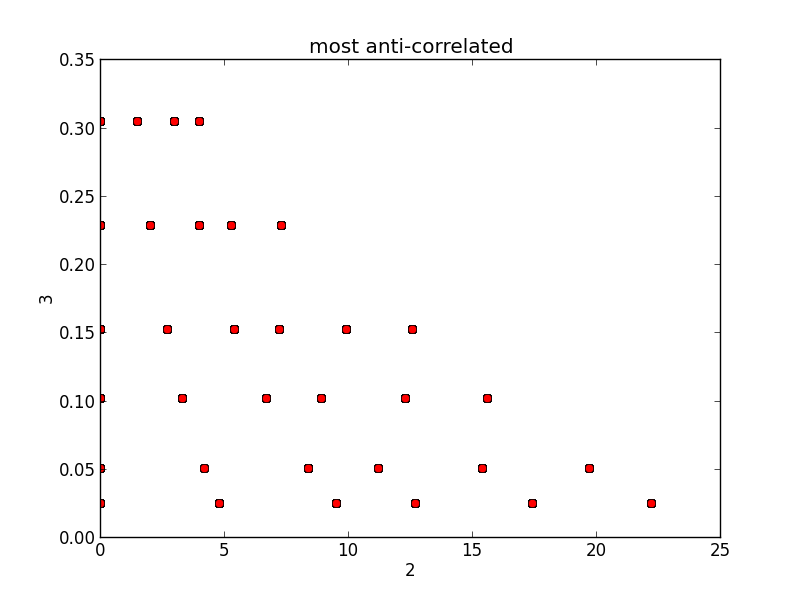
\includegraphics[scale=0.5]{figure_2}
\subparagraph{}The least correlated is col: (1, 3) , $cos(\theta)$ is  -0.003661, and the degree is 90.21
\subparagraph{}There is really weak correlation in this figure, compare with the figures above we cannot see a relation in this plot.
\subparagraph{}
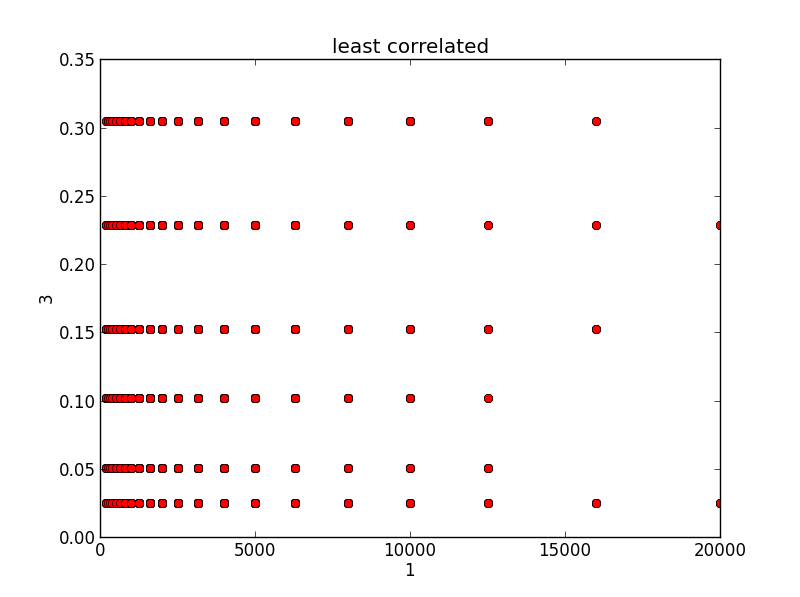
\includegraphics[scale=0.5]{figure_3}
\section{Part 2}
\subparagraph{}Eigenvectors $u_1$ and $u_2$($\epsilon = 0.0001$):
\subparagraph{}$u_1= 
\begin{bmatrix}1.00070832 \\
 -0.00051241  \\
 -0.00000011 \\
  0.00066074  \\
 -0.00000096  \\
 -0.00085559 
\end{bmatrix}
$
$u_2= 
\begin{bmatrix}-0.00049678\\
 0.0331156 \\
-0.00006833\\
 0.8849192 \\
 0.00001509\\
 0.08251522
\end{bmatrix}
$
\subparagraph{}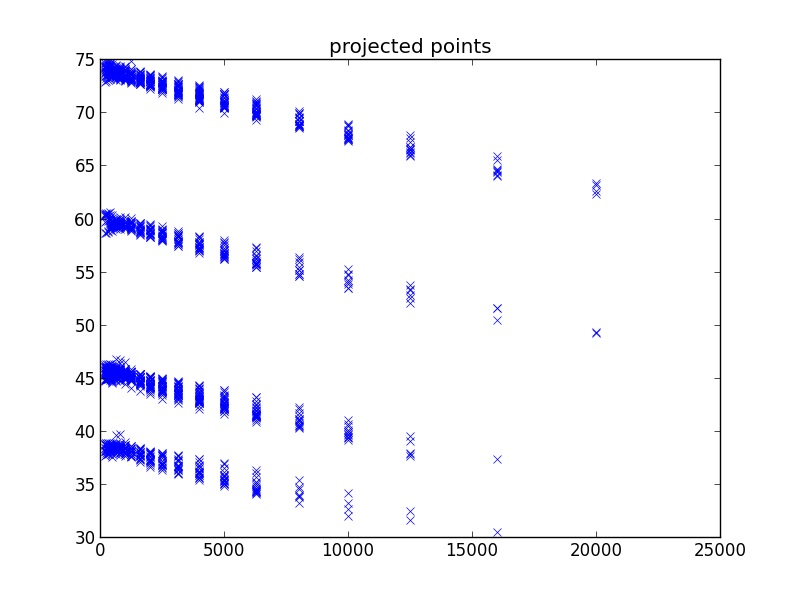
\includegraphics[scale=0.5]{figure_4}
\end{document}